\subsection{Mobil kliens megvaklósítása}
Ebben a fejezetben a mobil kliens implementációjának részleteit mutatjuk be. Sajnos előre nem látható és
technikai nehézségek miatt a megszabott határidőig nem sikerült a specifikációban előírt minden funkciót elkészíteni, 
itt csak a működő komponensek kerülnek bemutatásra.

A programban a következő főbb funkciók érhetők el: 
\begin{itemize}
    \item Regisztráció
    \item Bejelentkezés
    \item Művek böngészése
    \item Művek részleteinek megtekintése
    \item Művek olvasása
    \item Kedvelés küldése
    \item Hozzászólás írása
    \item korábbi privát üzenetek megtekintése
\end{itemize}

A mobilé architektúrája rétegekre bontható, ezek kifejtésében bemutatjuk nagyvonalakban a kód felépítését és a használt technológiákat.
 a használt androidos technológiákat.


\subsubsection{Adatlekérdezés (HTTP kliens)}
A mobil kliens a szerverrel való hálózati kommunikációt a Retrofit könyvtár segítségével valósítja meg.
A Retrofit egy nyílt forráskódú Android és Java HTTP-kliens, amely a REST API-k hívását teszi lehetővé.


\paragraph{REST API interfész}
Az API-hívások kezelésére a \texttt{WriterReaderApi} interfész definiálja a szerver által támogatott végpontokat. 
Az egyes metódusok Retrofit-es annotációkkal vannak ellátva, amelyek a megfelelő HTTP metódusokat és a végpontokat definiálják.
Az interfész nem tartalmazza az összes szerver által biztosított végpontot, hanem csak amelyek a mobil klens eddigi 
funkcióihoz szükségesek:

\begin{itemize}
    \item \textbf{Művek kezelése:}
    \begin{itemize}
        \item \texttt{getWorks}: Az összes mű lekérdezése.
        \item \texttt{getWork}: Egy adott mű részleteinek lekérdezése azonosító alapján.
    \end{itemize}
    \item \textbf{Felhasználók kezelése:}
    \begin{itemize}
        \item \texttt{getUsers}: Az elérhető felhasználók listázása.
        \item \texttt{getUser}: Egy adott felhasználó adatainak lekérdezése azonosító alapján.
        \item \texttt{getCurrentUser}: Az aktuálisan bejelentkezett felhasználó adatainak lekérdezése token alapján.
    \end{itemize}
    \item \textbf{Hozzászólások és kedvelések kezelése:}
    \begin{itemize}
        \item \texttt{postComment}: Hozzászólás küldése.
        \item \texttt{postLike}: Kedvelés hozzáadása.
        \item \texttt{deleteLike}: Kedvelés törlése.
    \end{itemize}
    \item \textbf{Hitelesítés:}
    \begin{itemize}
        \item \texttt{register}: Új felhasználó regisztrációja.
        \item \texttt{login}: Bejelentkezés a rendszerbe.
        \item \texttt{logout}: Kijelentkezés az aktuális munkamenetből.
    \end{itemize}
\end{itemize}

A HTTP kommunikációban JSON objektumokat használunk, melyeket kotlin osztályokra képződnek le
A JSON objektumok és Kotlin osztályok közti átalakítást a \textbf{Moshi} könyvtár segítségével végezzük el. 

\paragraph{Retrofit konfiguráció}
A REST API végpontok eléréséhez egy Retrofit klienst kell létrehozni, itt konfiguráljuk például az időtúllépési értékeket, a moshi JSON adaptert
és az alap URL-t a szerverhez, ami jelenleg \texttt{http://10.0.2.2}, ez egy alias és az android emulátoron a host gép címét jelenti.
A retrofit kliens a \texttt{WriterReaderApplication} osztályban az alkalmazáés indulásakor jön létre.

\subsubsection{Adatelérés (Repository)}

Az alkalmazás az adatelérésre egy a hálózati kommunikáció feletti absztrakciós réteget használ (\textbf{data access layer}), 
ami lényegeében egy \texttt{ApiMAnager} nevű wrapper osztály a Retrofit kliens és a hálózati hívások köré. Megkönnyíti a magasabb szintű kódból való használatot.
AZ adatelérési réteg két fontosabb feladata az API-hívások kezelése és a hibakezelés.
Az osztáy suspend fun metóduasi gondoskodnak arról,
hogy a hálózati hívások csak corutineokon belül történjenek, így ne blokkolják a UI szálat,
\paragraph{Hibakezelés} A válaszok kezeléséhez a \texttt{Retrofit Response} osztályt használja, 
amely tartalmazza a HTTP státuszkódot és a szerver által küldött adatokat. 
Minden API-hívás esetén figyelembe vesszük a lehetséges hibákat, mint például hálózati időtúllépést vagy nem várt szerverhibákat, 
hogy megfelelő visszajelzést adhassunk a felhasználónak. Az \texttt{ApiMAnager} metódusai onSuccess és onError callback 
függvényeket várnak paraméterként, amelyek a hálózati hívások végrehajtásakor hívódnak meg.

Az \texttt{ApiMAnager} osztályt az alkalmazás indulásakor pédányosítjuk így az egész alkalmazásban elérhető lesz.


\subsubsection{UI réteg (UI Layer)}

A alkalmazás egyes képernyőit MVI (Model-View-Intent) architektúra szerint valósítottuk meg.
Ennek az architektúrának 4 komponense van
\begin{itemize}
    \item \textbf{Model} 
    \item \textbf{Intent} 
    \item \textbf{View} 
    \item \textbf{View-Model}
\end{itemize}

\paragraph{Model}
A Model az alkalmazás állapotának (State) egy reprezentációja. Ez a komponens tartalmazza a képernyőhöz 
szükséges összes adatot és a felhasználói interakciók eredményét. 
Az állapot megváltozása új state objektum létrehozásával történik.

\paragraph{Intent}
Az Intent-ek képviselik a felhasználói interakciókat és a képernyő eseményeit (például: egy gomb lenyomása). 
Az Intent-ek explicit módon jelzik a ViewModel-nek, hogy milyen műveleteket kell végrehajtania.

\paragraph{View}
A View a Jetpack Compose deklaratív UI komponensei által megvalósított felhasználói felület.
Az composable elemek kizárólag a State alapján frissülnek.
A View nem tartalmaz logikát, hanem kizárólag az állapot megjelenítéséért felelős.


\paragraph{View-Model}
A ViewModel felel az Intent-ek feldolgozásáért és az állapot frissítéséért. 
Ez a komponens biztosítja a State folytonosságát és kezeli az üzleti logikát,
például hálózati kérések indítását.
A ViewModel figyeli az Intent-eket, végrehajtja a szükséges műveleteket, és az új állapotot a View felé közvetíti.




\subsubsection{Grafikus felhasználói felület}
Itt bemutatjuk a mobil kliens grafikus felhasználói felületét, az egyes képernyők szerint.
A \texttt{login} és \texttt{register} képernyőkön (\ref{fig:android_login}) a felhasználó bejelentkezhet, vagy új fiókot hozhat létre.
\begin{figure}[H]
    \centering
    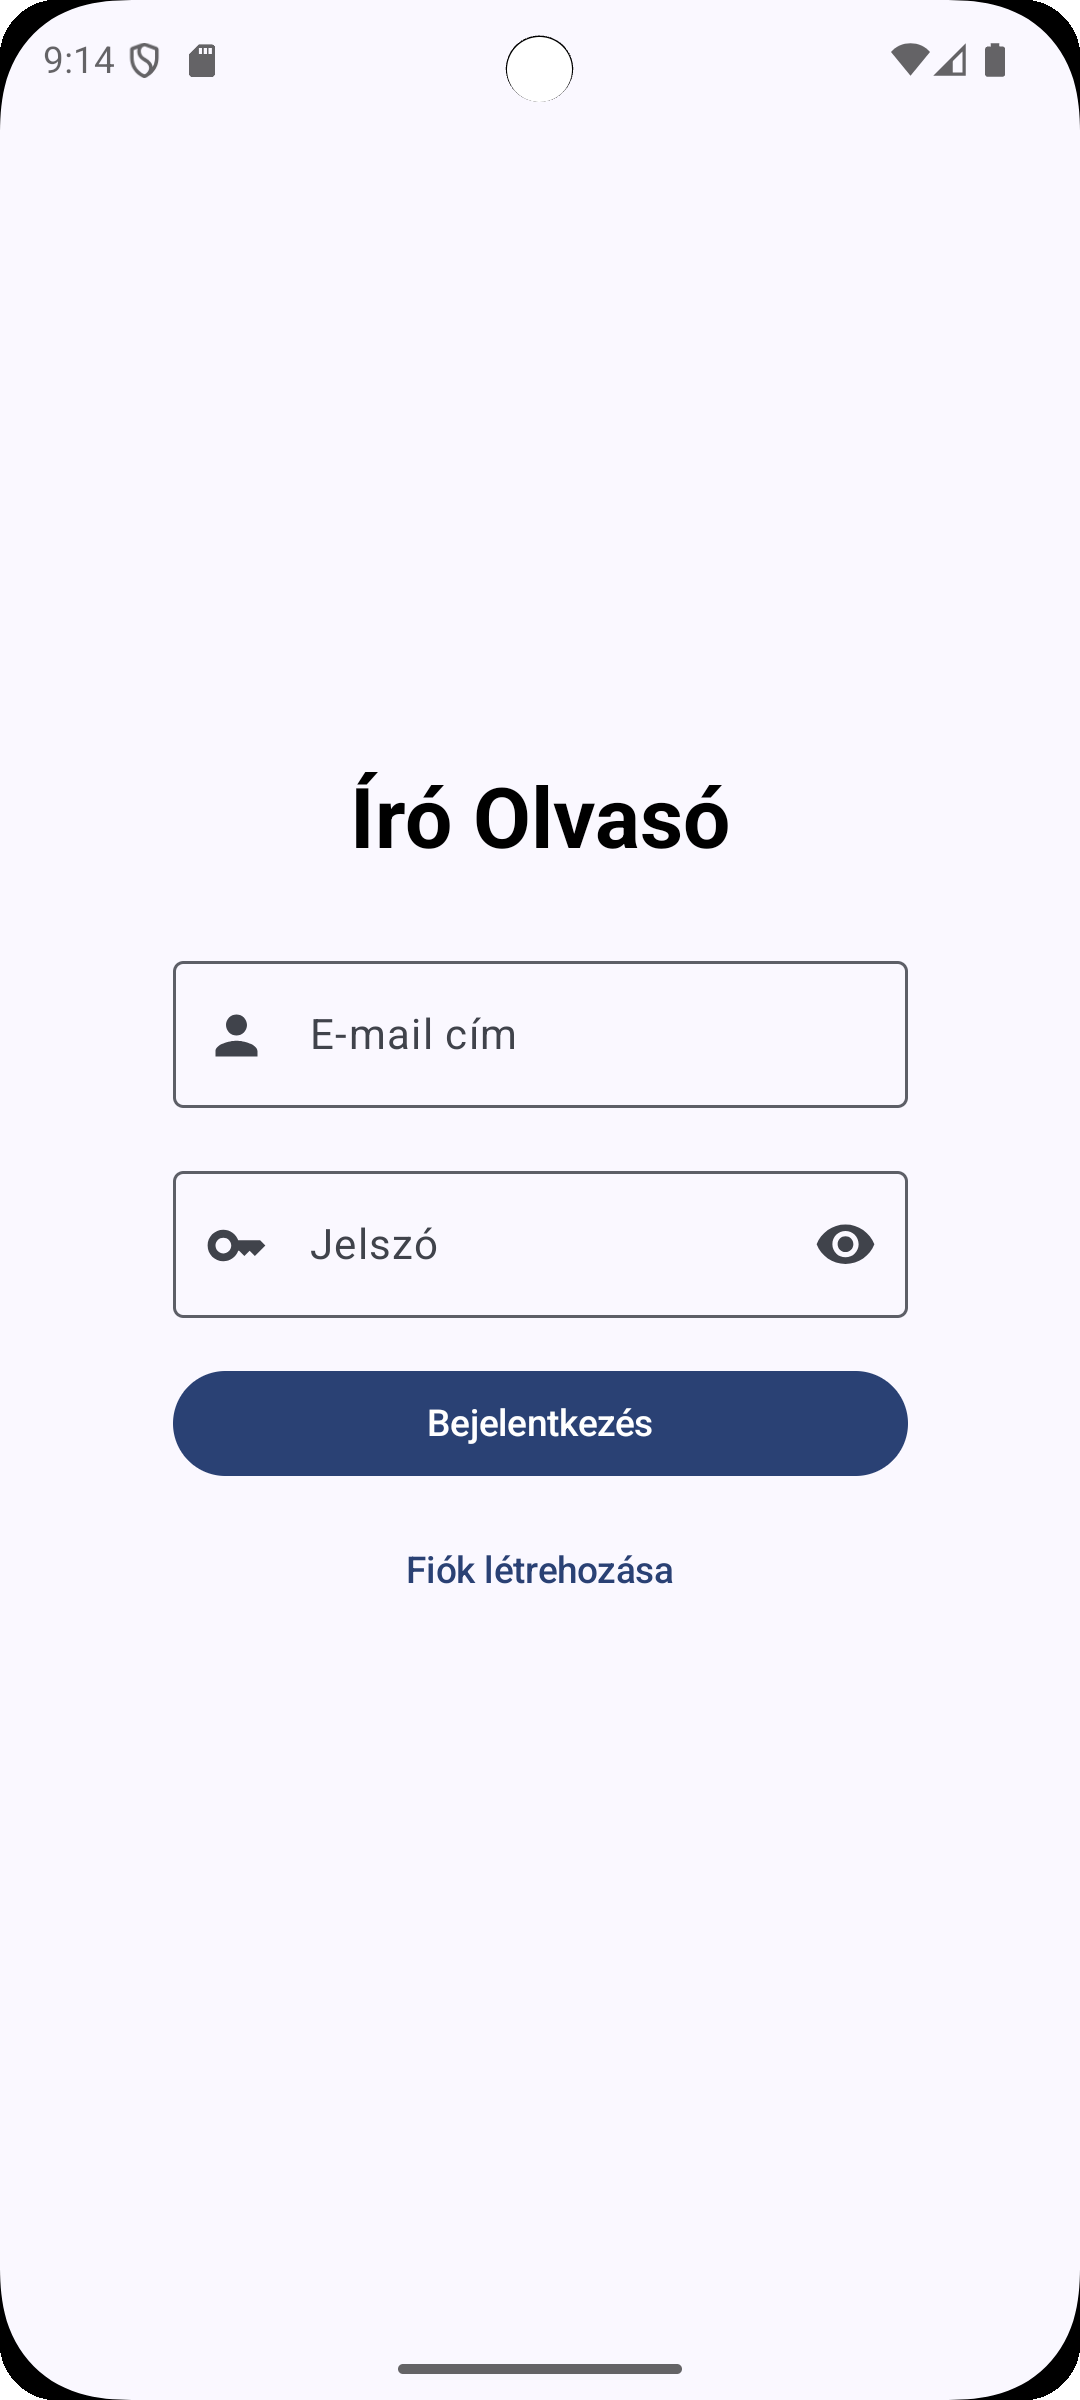
\includegraphics[width=0.25\textwidth]{figures/android_login.png}
    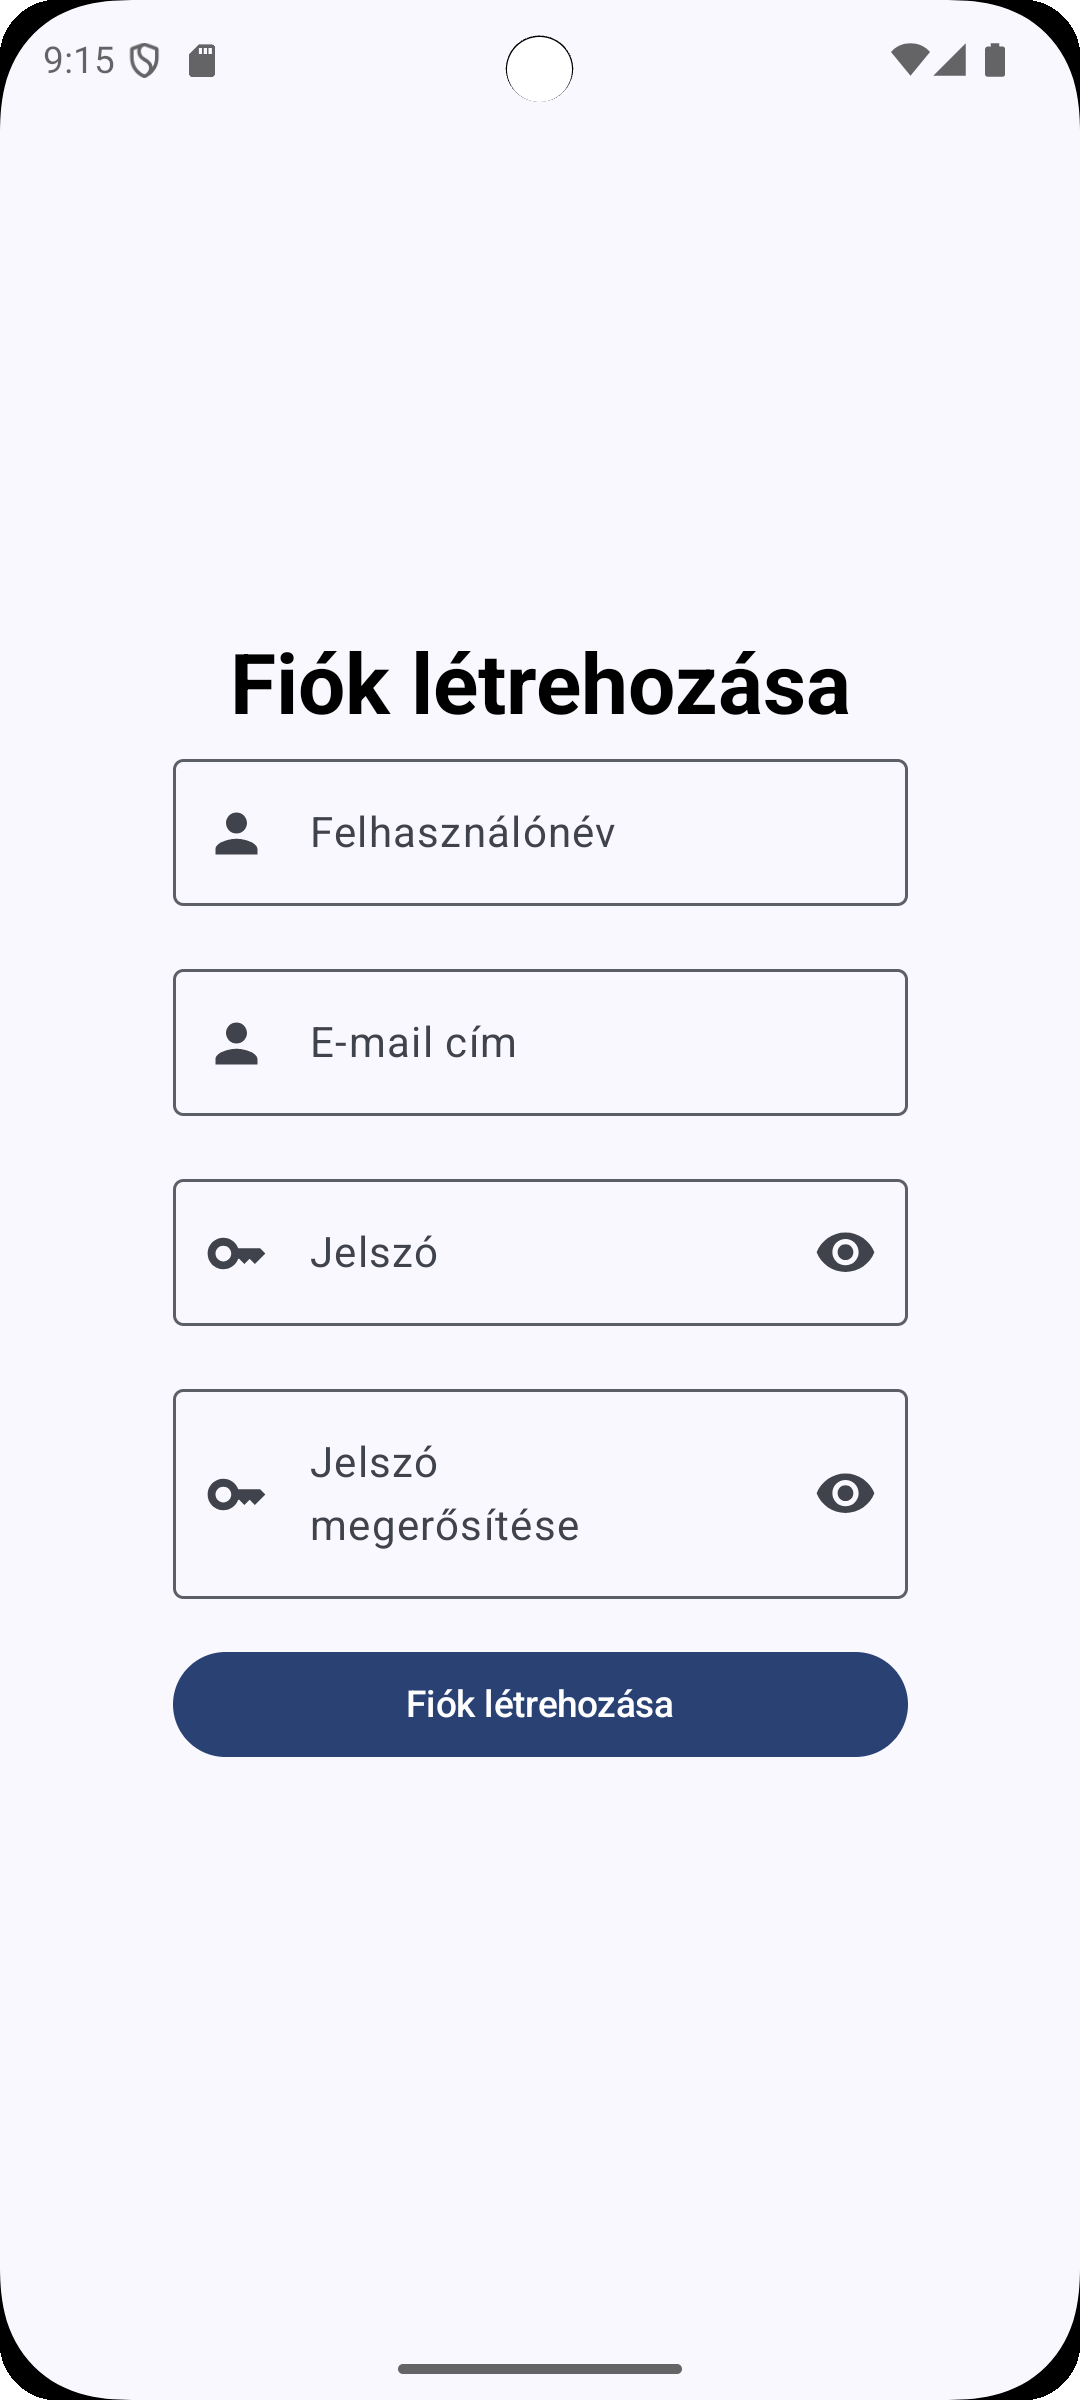
\includegraphics[width=0.25\textwidth]{figures/android_register.png}
    \caption{Bejelentkezési és regisztrációs képernyő}
    \label{fig:android_login}
\end{figure}

A sikeres bejelentkezés után a felhasználó a \texttt{home}  (\ref{fig:android_home}. ábra) képernyőre kerül, 
ahol a legfrissebb műveket láthatja, valamint kereshet a művek között cím vagy szerző alapján.
A képernyő alján navigációs sáv található, melyel a bejelentkerési és az üzenetek képernyőre lehet navigálni. 
(Sajnos az üzenetek képernyő még nincs implementálva.)

\begin{figure}[H]
    \centering
    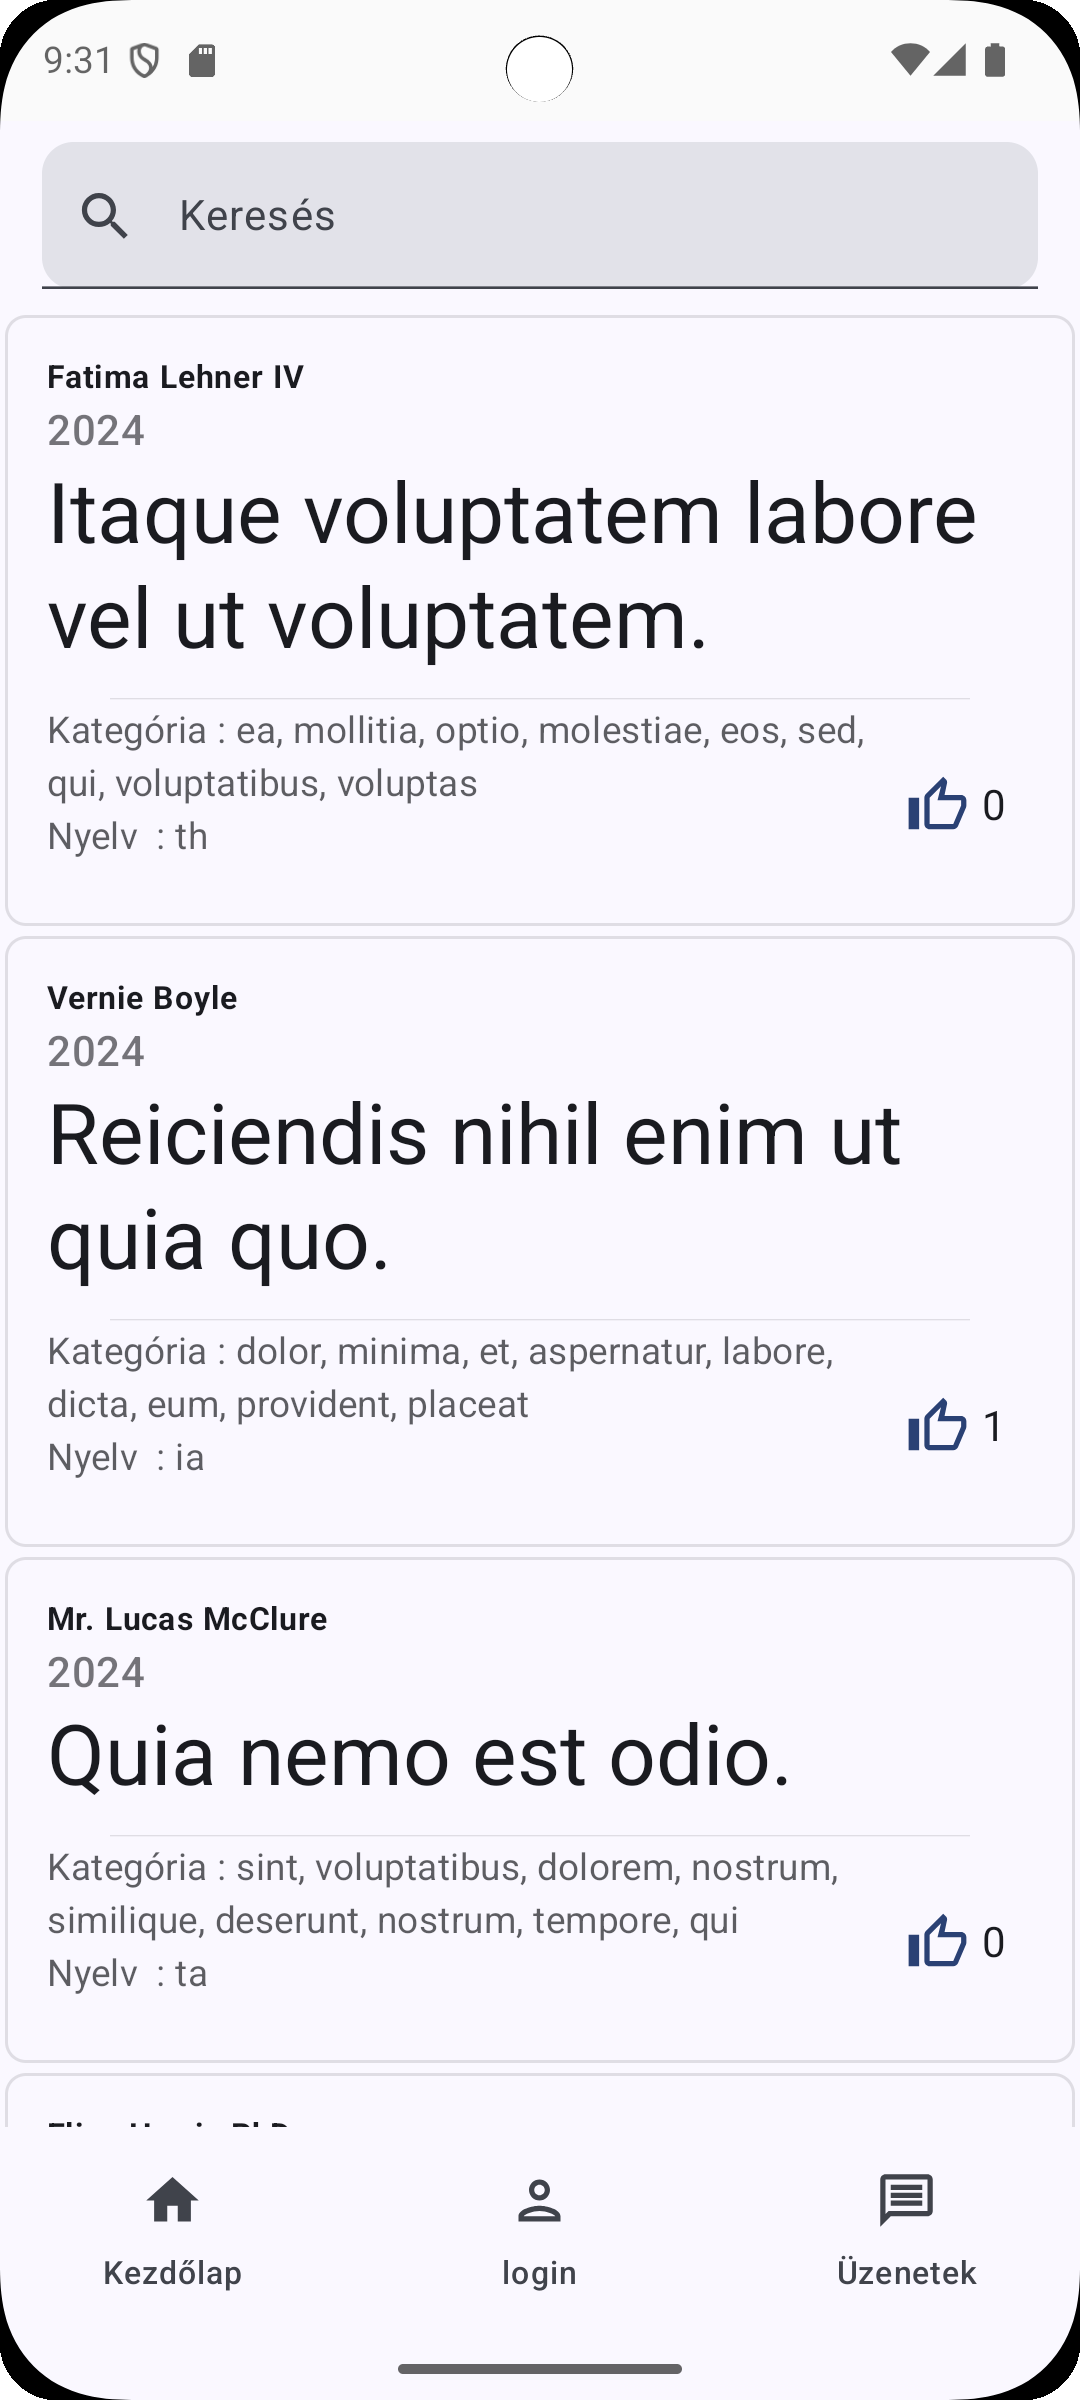
\includegraphics[width=0.25\textwidth]{figures/android_home.png}
    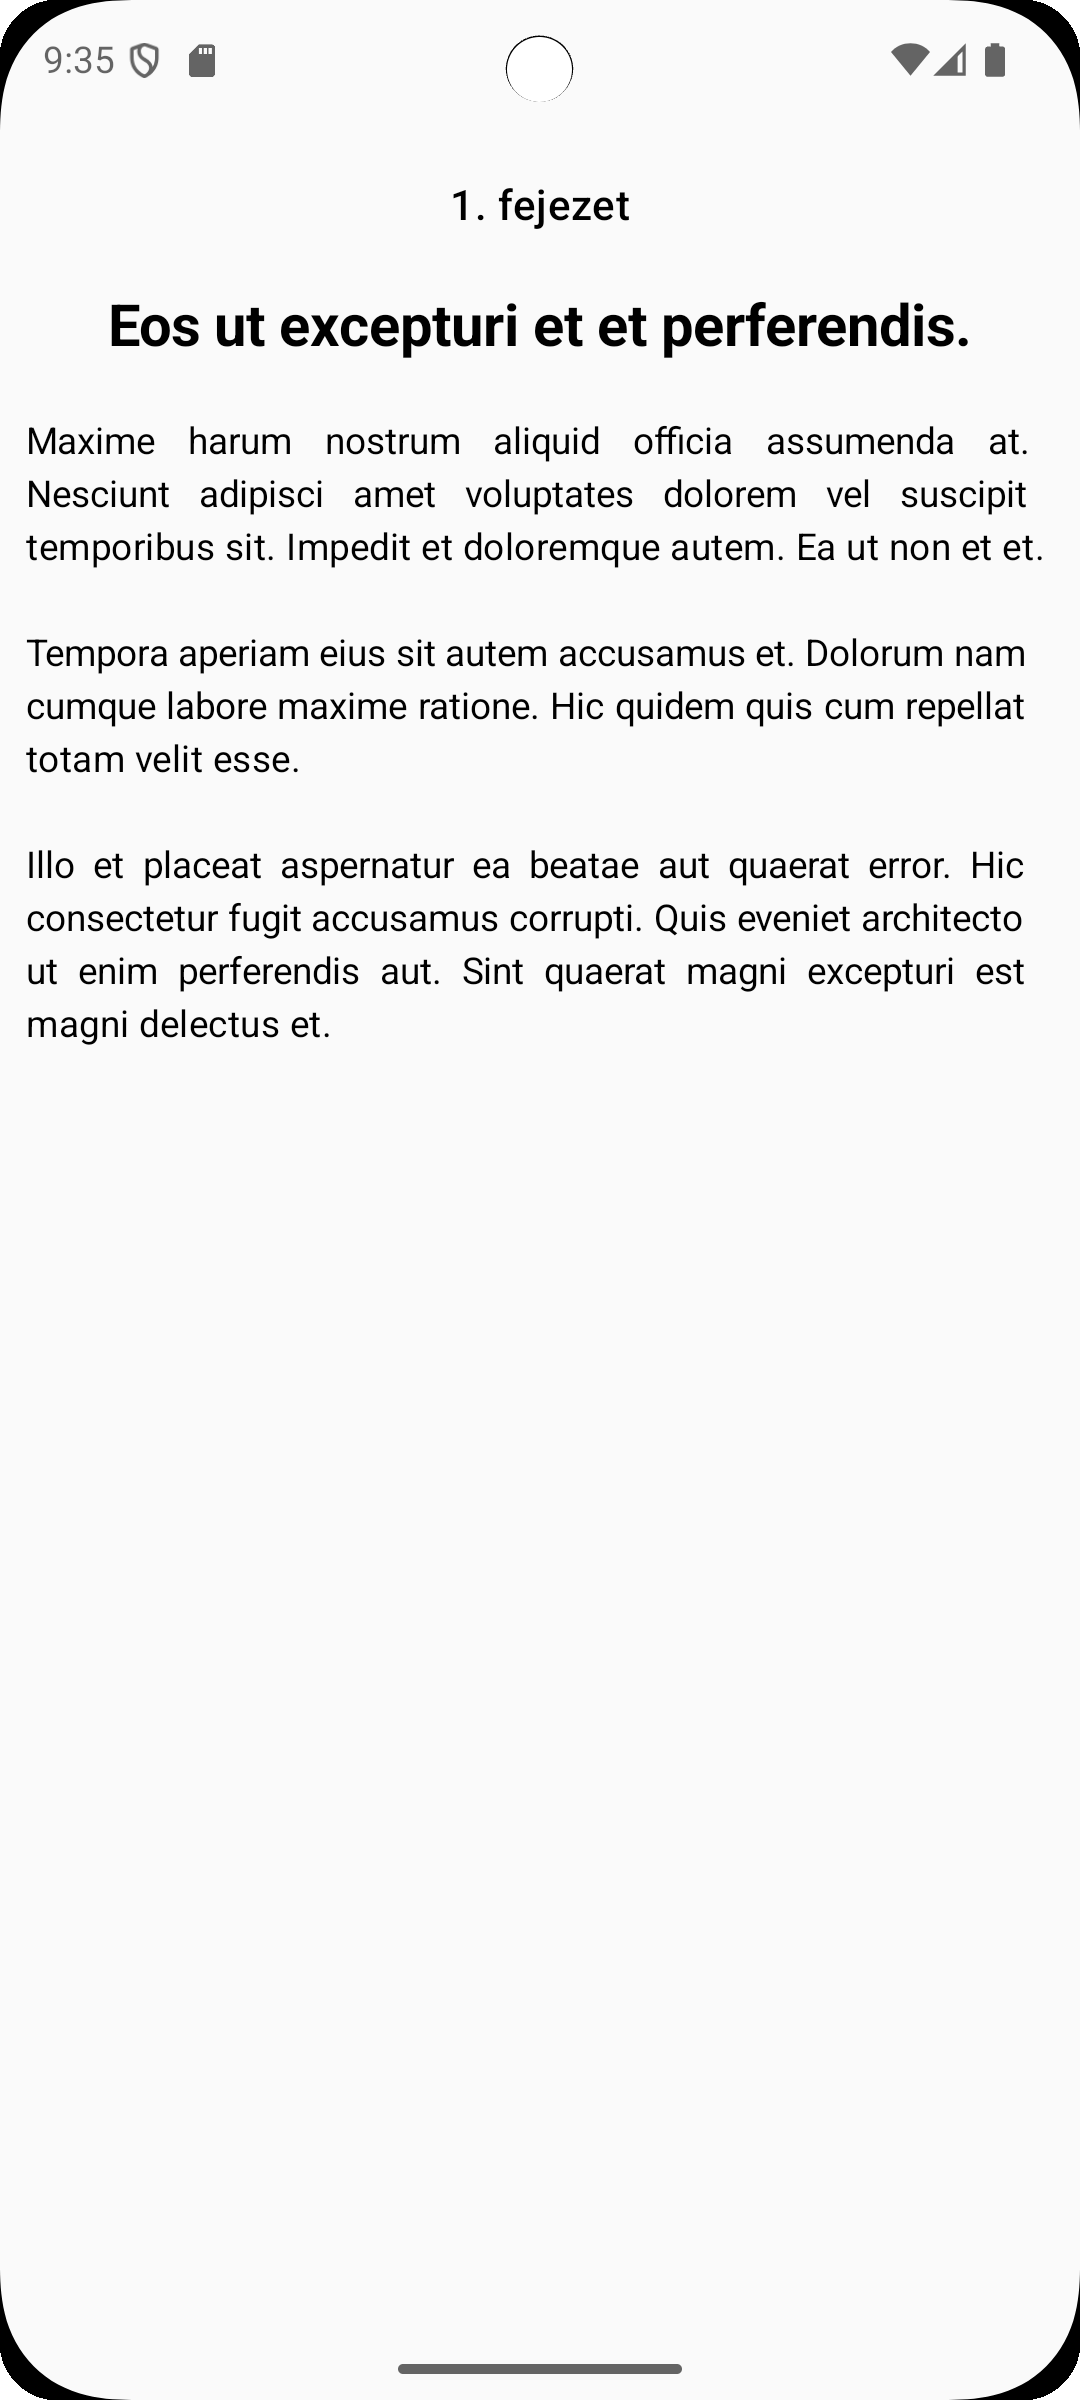
\includegraphics[width=0.25\textwidth]{figures/android_read.png}
    \caption{Kezdőképernyő és mű olvasása képernyő}
    \label{fig:android_home}
\end{figure}

Az egyes művekre kattintva a felhasználó a \texttt{work details} (\ref{fig:android_login}. ábra) képernyőre kerül, ahol a mű részleteit láthatja,
lájkolhatja, hozzászólást írhat.

\begin{figure}[H]
    \centering
    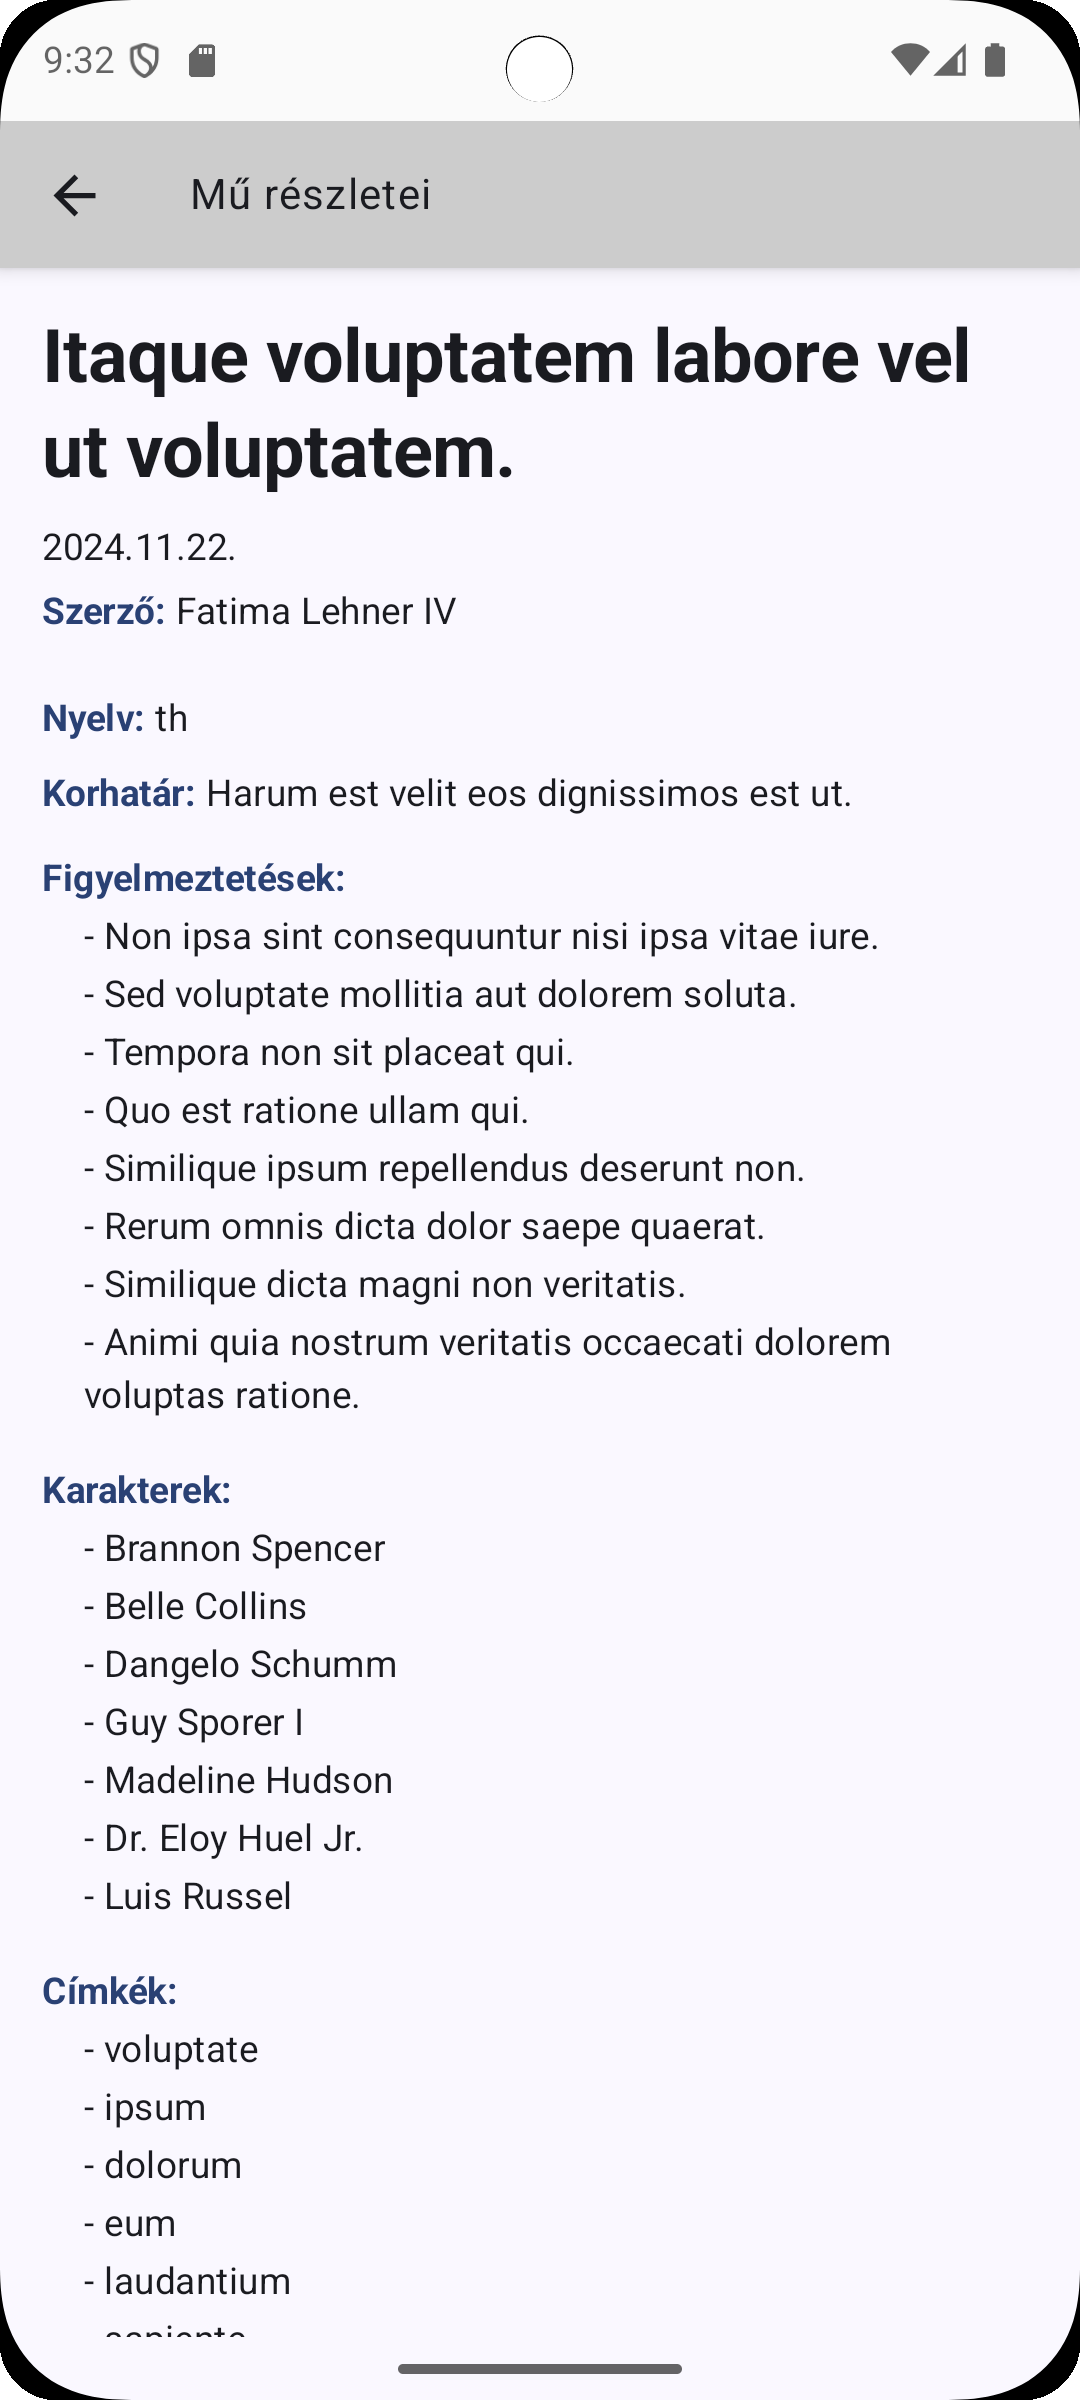
\includegraphics[width=0.25\textwidth]{figures/android_details1.png}
    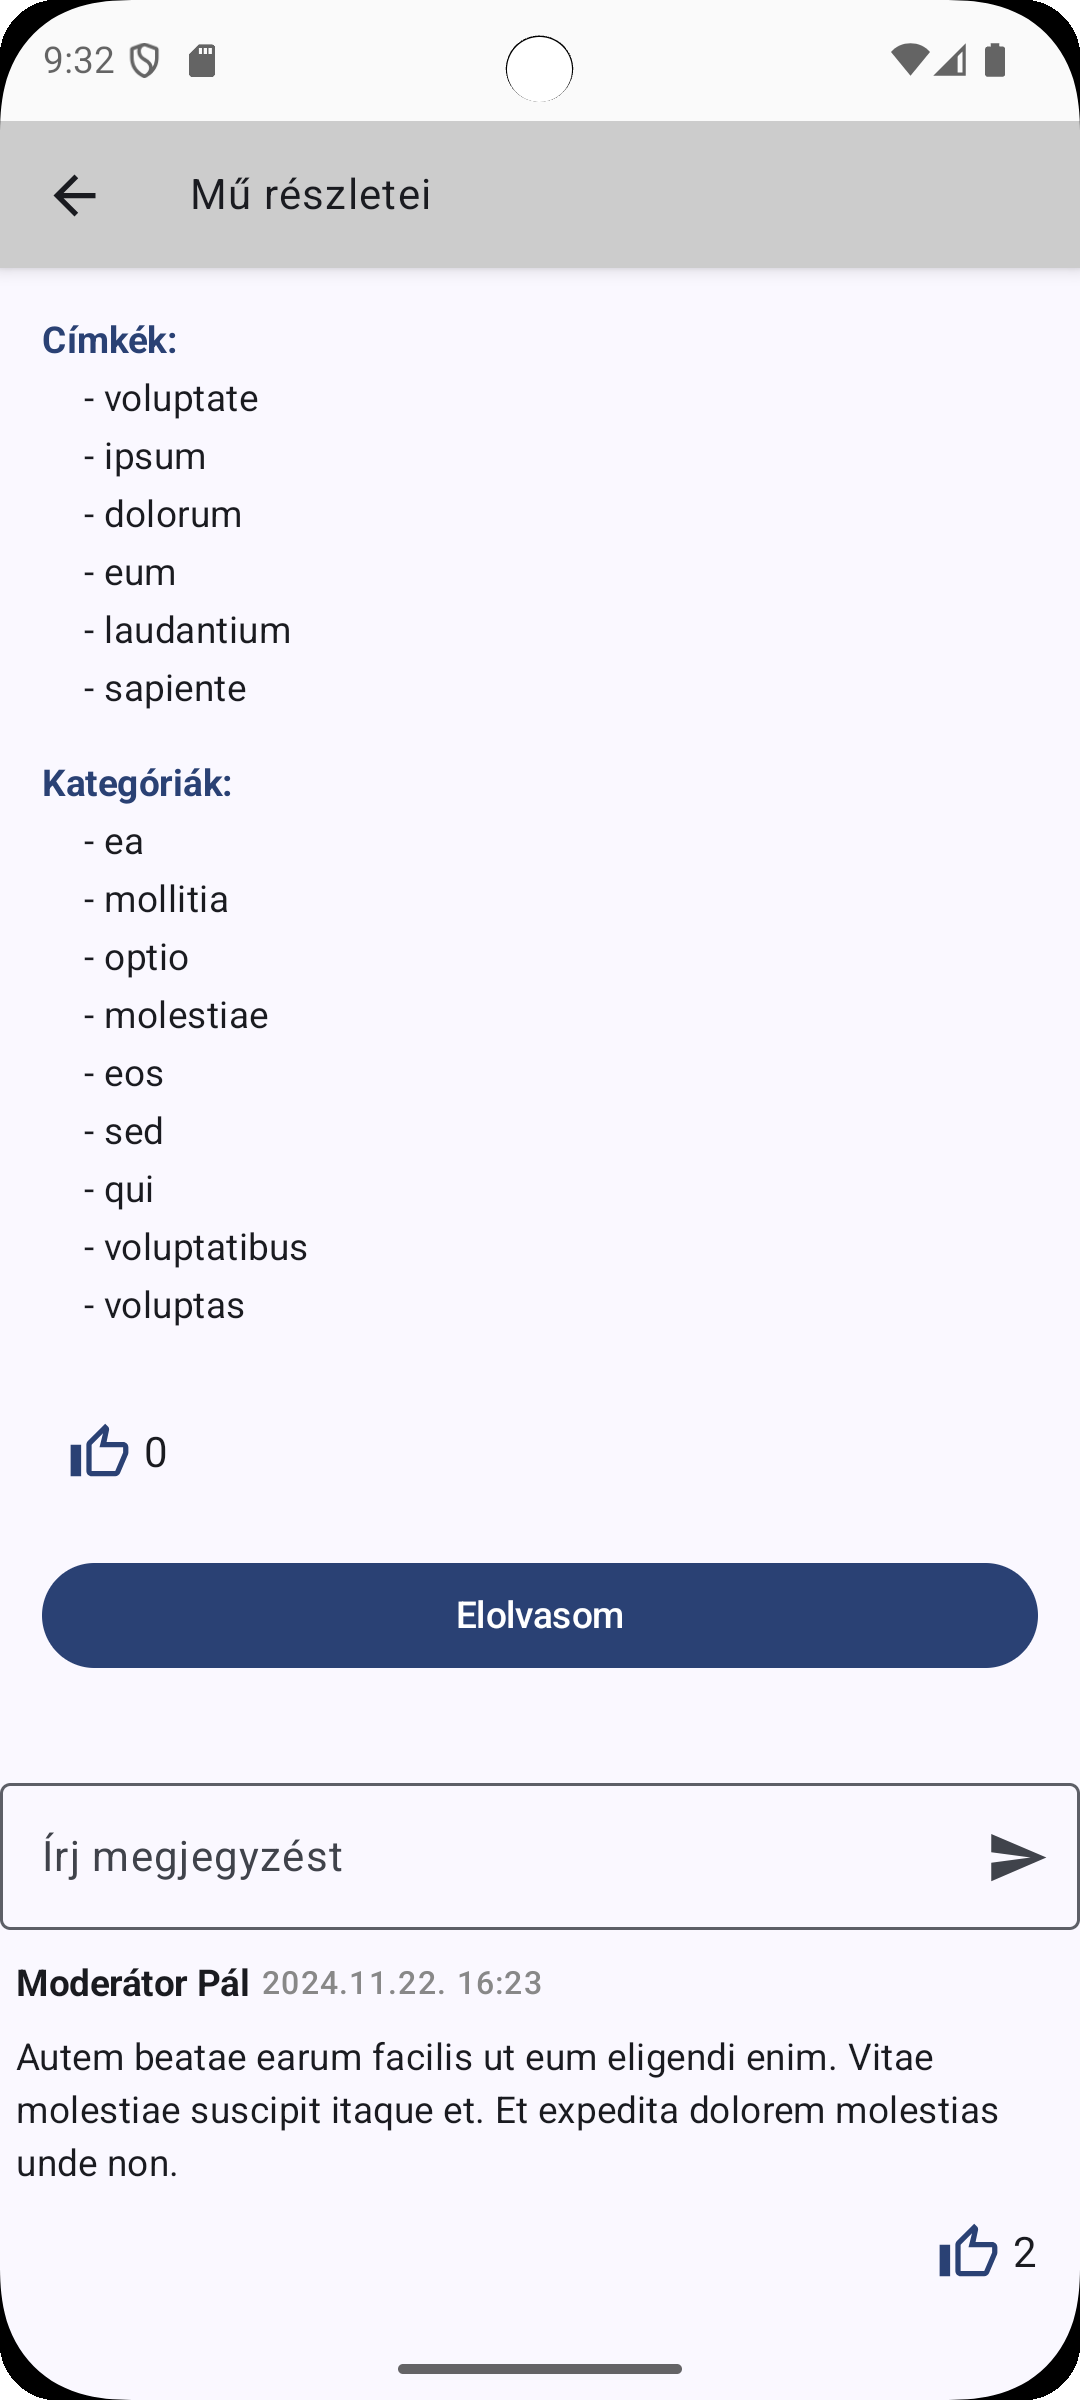
\includegraphics[width=0.25\textwidth]{figures/android_details2.png}
    \caption{Mű részletei képernyő}
    \label{fig:android_details}
\end{figure}

A mű olvasása gombra kattintva a felhasználó a \texttt{read work}  (\ref{fig:android_details}. ábra) képernyőre kerül, ahol a művet teljes terjedelmében elolvashatja.
Az olvasás teljes képernyős, az egyes fejezetek között lapozni lehet.

További funkciókat ellátó képernyők elkészítésére sajnos nem maradt időnk.
